%versi 2 (8-10-2016) 
\chapter{Pendahuluan}
\label{chap:intro}
   
\section{Latar Belakang}
\label{sec:label}

\textit{Outlook.com}\footnote{https://outlook.live.com/} adalah sebuah kumpulan aplikasi berbasis \textit{web} seperti \textit{webmail}, \textit{contacts}, \textit{tasks}, dan \textit{calendar} dari \textit{Microsoft}. Fitur \textit{calendar} sendiri pertama dirilis pada 14 Januari 2008 dengan nama \textit{Windows Live Calendar}. Fitur \textit{calendar} yang dimiliki oleh \textit{Outlook.com Calendar} sendiri memiliki tampilan yang mirip dengan aplikasi kalender \textit{desktop} pada umumnya. Seperti layaknya kalender digital pada umumnya, aplikasi \textit{Outlook.com Calendar} juga bisa menambahkan, menyimpan, dan memodifikasi \textit{event-event} yang dimasukkan oleh pengguna dan bisa dibuka dimana saja karena bersifat \textit{online}. 

\textit{Slack}\footnote{https://slack.com/} adalah alat dan layanan kolaborasi tim berbasis \textit{cloud}. \textit{Slack} merupakan singkatan dari ``\textit{Searchable Log of All Conversation and Knowledge}''. Cara melakukan kolaborasi di aplikasi \textit{Slack} sendiri adalah dengan cara komunitas, grup, atau tim bergabung ke dalam URL yang spesifik yang disebut dengan \textit{workspace}. \textit{Room chat} yang terdapat di dalam \textit{workspace} biasa disebut dengan \textit{Channel}. Ada 2 jenis \textit{channel} di dalam \textit{workspace} yang ada di aplikasi \textit{Slack} yaitu \textit{Public Channel} dan \textit{Private Channel}. Pada \textit{Public Channel}, seluruh anggota dari tim atau komunitas bisa masuk dan bergabung untuk berkomunikasi di \textit{channel} tersebut. Tetapi pada \textit{Private Channel}, hanya anggota yang diizinkan, ditambahkan, dan diundang oleh admin atau pembuat \textit{channel} sajalah yang bisa ikut berkomunikasi di dalam \textit{channel} tersebut. Pada setiap \textit{workspace} dapat ditambahkan dan dipasangkan aplikasi penyokong lainnya seperti contohnya adalah \textit{Trello}, \textit{Github}, \textit{Google Drive}, dan banyak aplikasi lainnya yang bisa digunakan untuk membantu para partisipan di dalam \textit{workspace} tersebut. 

Pada \textit{Slack} terdapat status pengguna yang bisa diganti oleh pengguna tersebut untuk menggambarkan keadaan pengguna saat ini. Nilai \textit{default} dari status ini adalah tersedia, tetapi \textit{Slack} sudah menyediakan beberapa pilihan status seperti ``\textit{In a meeting}'', ``\textit{Commuting}'', ``\textit{Out sick}'', ``\textit{Vacationing}'', dan ``\textit{Working remotely}'' seperti yang terdapat pada contoh gambar \ref{fig:status_list_slack}. Selain itu, \textit{Slack} juga menyediakan pilihan untuk pengguna yang mengisi statusnya sendiri. Dengan adanya fitur status di dalam aplikasi \textit{Slack}, maka hal itu membantu mendeskripsikan keadaan yang sedang dialami oleh pengguna saat itu. Status hanya berupa keterangan di akun pengguna dan tidak berdampak kepada fitur lainnya seperti contohnya fitur obrolan. Yang menjadi latar belakang dirancangnya perangkat lunak ini yaitu terkadang pengguna lupa untuk mengganti status menjadi ``\textit{In a meeting}'' saat pengguna memiliki jadwal untuk melakukan \textit{meeting}, sehingga status di pengguna masih terlihat tersedia oleh \textit{user} lain yang membuat tidak mengetahui pengguna sedang dalam keadaan \textit{meeting}. Di saat seperti ini, kemungkinan untuk \textit{meeting} terganggu oleh adanya \textit{chat} yang masuk lewat \textit{Slack} pun cukup tinggi. Tetapi status hanya membantu mendeskripsikan keadaan yang sedang dialami oleh pengguna saat itu dan tidak memblokir chat masuk kepada pengguna. 

\begin{figure}[h]
  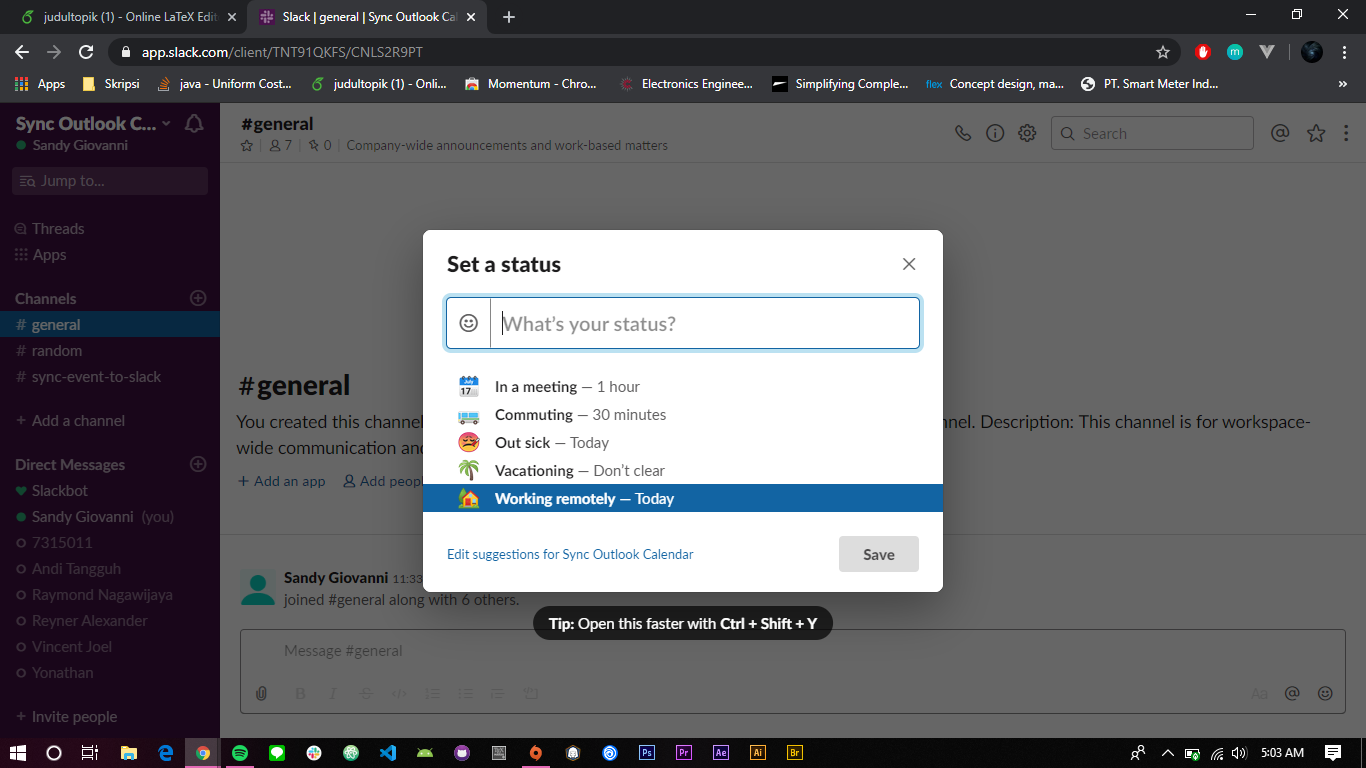
\includegraphics[width=10cm]{./Gambar/list_status.png}
  \centering
  \caption{\textit{List} status yang disediakan sebagai pilihan di \textit{Slack}.}
  \label{fig:status_list_slack}
\end{figure}

Pada skripsi ini dibuat perangkat lunak yang membaca jadwal dari pengguna yang dicantumkan di aplikasi \textit{Outlook.com Calendar}, lalu akan di integrasikan ke aplikasi \textit{Slack} dengan mengubah status di dalam aplikasi \textit{Slack} sesuai dengan jadwal yang telah didapatkan dari data di \textit{Outlook.com Calendar} dari pengguna. 

Perangkat lunak ini dibuat menggunakan \textit{Node.js}\footnote{https://nodejs.org} dan memiliki 2 fungsi utama yaitu yang pertama adalah membaca dan mencatat jadwal dari \textit{Outlook.com Calendar} yang membutuhkan adanya \textit{Outlook.com Calendar API}. Lalu fungsi kedua yaitu mengubah status ke aplikasi \textit{Slack} dengan menggunakan \textit{Slack API}. Kedua fungsi dari perangkat lunak ini dijalankan secara berkala sehingga perubahan status yang terjadi pada aplikasi \textit{Slack} tidak terjadi secara \textit{real-time} tetapi berkala setiap 10 menit sekali dilakukan penjalanan dari fungsi perangkat lunak ini.  

\textit{API} atau \textit{Application Programming Interface} adalah sebuah \textit{interface} yang memungkinkan antara 2 aplikasi atau lebih saling berinteraksi. \textit{Outlook Calendar} sendiri memiliki \textit{API} yang berpusat pada \textit{Microsoft Graph API}, lalu pada aplikasi \textit{Slack} juga sudah disediakan \textit{API} sehingga untuk mengkomunikasikan antara kedua aplikasi ini bisa menggunakan \textit{API} dari masing-masing aplikasi yang sudah disediakan. 

\section{Rumusan Masalah}
\label{sec:rumusan}
Pada perangkat lunak ini, terdapat rumusan masalah sebagai berikut:
\begin{enumerate}
	\item Bagaimana cara mendapatkan data \textit{event} dari \textit{Outlook.com Calendar}?
	\item Bagaimana mengubah status pada aplikasi \textit{Slack} menggunakan \textit{Slack} API?  
	\item Bagaimana cara membuat program agar dapat mengubah status pada aplikasi \textit{Slack} di jadwal yang telah didapat dari aplikasi \textit{Outlook.com Calendar}? 
	
\end{enumerate}

\section{Tujuan}
\label{sec:tujuan}
Adapun pada perangkat lunak ini memiliki tujuan sebagai berikut:
\begin{enumerate}
	\item Mengetahui cara mendapatkan data \textit{event} dari \textit{Outlook.com Calendar}.   
	\item Mengetahui cara mengubah status pada aplikasi \textit{Slack} menggunakan \textit{Slack} API. 
	\item Membuat program agar dapat mengubah status pada aplikasi \textit{Slack} di jadwal yang telah didapat dari aplikasi \textit{Outlook.com Calendar}.  
\end{enumerate}

\section{Batasan Masalah}
\label{sec:batasan}
Perancangan perangkat lunak ini dibuat berdasarkan batasan-batasan sebagai berikut: 
\begin{enumerate}
	\item Perangkat lunak ini dijalankan secara berkala sehingga tidak dapat mengubah status secara \textit{real-time}. 
	\item Hanya berlaku untuk setiap satu pengguna terhubung dengan satu \textit{workspace} saja di dalam \textit{Slack}(Tidak berlaku satu pengguna ke banyak \textit{workspace}). 
\end{enumerate}

\section{Metodologi}
\label{sec:metlit}
Berikut adalah metodologi yang akan digunakan dalam penelitian ini: 
\begin{enumerate}
	\item Melakukan studi literatur tentang \textit{Outlook.com Calendar}, \textit{Slack}, dan juga \textit{Node.js}.
	\item Menggunakan aplikasi \textit{Slack} di lingkungan tempat penulis melakukan magang. 
	\item Melakukan analisis cara melakukan \textit{synchronize} dengan aplikasi \textit{Outlook.com Calendar} secara berkala. 
	\item Merancang bagian dari perangkat lunak yang akan mengambil data-data \textit{event} dari \textit{Outlook.com Calendar} dan yang bertugas untuk mengubah status pada \textit{Slack} saat waktu sesuai dengan jadwal yang sudah tercatat dari \textit{Outlook.com Calendar}.
	\item Mengimplementasi bagian pengambilan data dari \textit{Outlook.com Calendar} dan juga bagian mengatur status pada \textit{Slack} sesuai jadwal yang telah diambil kepada perangkat lunak Integrasi \textit{Outlook.com Calendar} dengan \textit{Slack} serta melakukan pengujian terhadap fitur yang telah diimplementasikan.
	\item Penulisan dokumen. 
\end{enumerate}

\section{Sistematika Pembahasan}
\label{sec:sispem}
Setiap bab dalam penelitian ini akan memiliki sistematika pembahasan yang dijelaskan ke dalam poin-poin sebagai berikut:
\begin{enumerate}
	\item Bab 1: Pendahuluan, yaitu menjelaskan gambaran umum dari penelitian ini yang berisi tentang latar belakang, rumusan masalah, tujuan, batasan masalah, metodologi, dan sistematika pembahasan.
	\item Bab 2: Dasar Teori, yaitu menjelaskan dan membahas teori yang dibutuhkan untuk melakukan penelitian ini. Meliputi tentang \textit{Outlook.com Calendar API}, \textit{Slack API}, dan \textit{Node.js}. 
	\item Bab 3: Analisis, yaitu membahas mengenai analisis masalah. Berisi tentang analisis cara pengambilan data dari \textit{Outlook.com Calendar}, dan proses pengubahan status menggunakan program pada \textit{Slack}.
	\item Bab 4: Perancangan, yaitu membahas mengenai perancangan aplikasi untuk melakukan sinkronisasi antara \textit{Outlook.com Calendar} dengan \textit{Slack}. 
	\item Bab 5: Implementasi dan Pengujian, yaitu membahas mengenai implementasi dari perangkat lunak yang telah dirancang dan juga pengujian perangkat lunak tersebut.   
	\item Bab 6: Kesimpulan dan Saran, yaitu berisi tentang kesimpulan dari penelitian ini dan juga saran yang dapat diberikan untuk penelitian selanjutnya.  
\end{enumerate}